\documentclass{report}


% Preamble for english writing
\usepackage[utf8]{inputenc}
\usepackage[T1]{fontenc}
\usepackage{amsmath}
\usepackage{amsfonts}
\usepackage{amssymb}
\usepackage{amsthm}
%\usepackage{algorithmic}
\usepackage{color}
\usepackage{enumerate}
\usepackage{stmaryrd}
\usepackage{hyperref}
\usepackage{graphicx}

%\usepackage{tkz-graph}

%\usepackage[nottoc, notlof, notlot]{tocbibind}

%%%%%%%%%%%%%%%%%%%%%%%%%%%%%%%%%%%%%%%%%%%%%%%%%%%%%%%%%%%%%%%%%%%
%Commandes ajoutées
%%%%%%%%%%%%%%%%%%%%%%%%%%%%%%%%%%%%%%%%%%%%%%%%%%%%%%%%%%%%%%%%%%%

%ensmembles
\newcommand{\N}{\mathbb{N}}
\newcommand{\Z}{\mathbb{Z}}
\newcommand{\Q}{\mathbb{Q}}
\newcommand{\R}{\mathbb{R}}


\newcommand{\intv}[2]{\llbracket #1, #2 \rrbracket} %intervalle d'entiers
\newcommand{\bracket}[1]{{\langle #1 \rangle}} %parenthèses angulaires
\newcommand{\gO}{\mathcal{O}} %grand O
\newenvironment{itemiz}{\renewcommand\labelitemi{$\blacktriangleright$}\begin{itemize}}{\end{itemize}}

\newcommand{\rg}{\text{rg}}
\newcommand{\bad}{\textbf{/!\backslash}}

\newcommand{\crk}{\text{cut-rank}}

\newcommand{\ie}{\emph{i.e.}\ }
\newcommand{\eg}{\emph{e.g.}\ }
\newcommand{\cf}{\emph{c.f.}\ }

% Theorems etc.
\newtheorem{Thm}{Theorem}[section]
\newtheorem{Cor}[Thm]{Corollary}
\newtheorem{Lem}[Thm]{Lemma}
\newtheorem{Pro}[Thm]{Proposition}

\theoremstyle{remark}
\newtheorem{Rem}[Thm]{Remark}
\newtheorem{Not}[Thm]{Notation}
\newtheorem{Exa}[Thm]{Example}

\theoremstyle{definition}
\newtheorem{Def}[Thm]{Definition}

\newcommand{\mytitle}[1]{
\begin{center}
\vspace{7cm}
\hrule
\vspace{0.5cm}
\huge{\textsc{#1}}
\vspace{0.5cm}
\hrule
\vspace{1cm}
\end{center}}




\title{Machine Learning Project Report\\\textbf{Evolutionnary Computing\\on Turing machines}\\{\Large Solving the Busy Beaver Problem}}
\author{Jean-Florent Raymond\\\href{mailto:jean-florent.raymond.8795@student.uu.se}{\texttt{jean-florent.raymond.8795@student.uu.se}} \and Emilio Del Tessandoro\\
  \href{mailto:emilio.del_tessandoro.4062@student.uu.se }{\texttt{emilio.del\_tessandoro.4062@student.uu.se }}}
\date{\today}

\begin{document}
\maketitle

\begin{abstract}

  Busy beavers are Turing machines that performs ``the most operations'' before halting among all Turing machines with the same alphabet and number of states. It have been introduced in 1962 by Tibor Radó and Shen Lin, and there is theoretical issues that make finding the busy beavers a difficult problem.
The goal of our project was to see if evolutionary computing techniques are suitable for finding busy beavers, and we found that <!!!what we found>.

\end{abstract}

\chapter{Introduction}
\label{chap:intro}

Given an alphabet and a set of states, we want to find a Turing machine that performs the most shifts before halting. The usual approaches \cite{rado} to this problem are
\begin{itemize}
\item running different machines (eventually all is there is not too much) until it halts (if so) and keeping the best ;
\item detecting patterns on the tape that means that the machine will stop after a certain number of shifts.
\end{itemize}
These methods can be improved using techniques of loop detection or by predicting the configuration of the machine in a certain number of step given the tape and the transition table.

Our approach is different. We use a genetic algorithm to find busy beavers. We have a population of Turing machines and we perform operations on it until it lead to a busy beaver.

For this, we designed and wrote a program to handle and execute Turing machines, and a program to simulate evolution on a population of Turing machines.

With this method, we were able to find busy beavers for small machine sizes. We know that this is really busy beavers because maximum number of steps before halting is known for theses machine sizes. When the machine size grows, to search space become huge and we were out of time to run the experiments long enough to be able to find good candiates. However, no busy beaver is know for these sizes at the time of writing this paper. Only lower bounds are know for some sizes.


% Operations are only performed on transition tables because it would be nonsense to mix or change the tapes. In the same time we perform operations on the population, we run the machines for a few steps each time, then we have an idea of how long the machines can run. We evaluate a fitness function on these machines, which is function of the number of steps performed so far. So we can use this fitness value to decide which indiviuals 


% Finding busy beavers becomes quickly difficult when the alphabet size and the number of states grows because of the huge number of different machines and because of the halting problem, which make us unable to know if a given machine will halt or no. Currently, busy beavers are only known for small alphabets and number of states and have only be studied by detecting ``good'' patterns on the tape or by executing different machines until it halts (if so).
% A big issue is the computation of the fitness function, since we don't know and cannot know when a machine will halt (if it halts).

\chapter{Definitions and Conventions}
\label{chap:pre}

\section{Machines}

We assume that the reader is familiar with the notion of Turing machine. In this paper, we only use deterministic Turing machines so it is what we mean when we use the expression \emph{Turing machine}. The tape is infinite on both sides.

\paragraph{Symbols}
We only deal with Turing machines with a finite alphabet. So we can represent it by an initial segment of $\N$. Furthermore, we choose that $0$ is the blank symbol. Our input alphabet is always $\{0\}$ since we only start on blank tapes. 

\paragraph{States}
Turing machines we are working with have a finite set of states and only one halt state.
 Except where otherwise stated, when we write that a Turing machine have $n$ states, we mean $n$ \emph{operational} states, \ie states that are not halt states. We use to use the letter $m$ to denote the cardinality of the alphabet and the letter $n$ to denote the cardinality of the operational states set.

 Let $\mathcal{T}_{m,n}$ be the set of deterministic Turing machines with an alphabet of $m$ symbols which uses $n + 1$ states, one of whom is the halt state, reached at most one time (because then the machine halts). Let  $\mathcal{T} = \cup_{n,m \in \N} \mathcal{T}_{n,m}$.

Since we only deals with finite states sets, we choose without loss of generality to represent any state set by an initial segment of $\N$ of the corresponding size. For instance, a machine $M \in \mathcal{T}_{m,n}$ have $\intv{0}{n}$ as states set and $\intv{0}{m-1}$ as alphabet.

What is more, since states names are interchangeable (with modifying the transition table according to this change), we choose that the start state is always state $0$ and the (maybe never reached) halting state is always state $n$.



\paragraph{Machines}
All the assumptions we do simplifies the representation of machines so we can now define if easily.

\begin{Def}[Turing machine]

A \emph{Turing machine} $M$ of $\mathcal{T}$ is a triple $(m,n,\delta)$ where 
\[
\left \{
\begin{array}{l}
  n \in \N^*\\
  m \in \N^*\\
  \delta : \intv{0}{m-1} \times \intv{0}{n-1} \to \intv{0}{m-1} \times \intv{0}{n} \times \{0,1\}
\end{array}
\right .
\]
The function $\delta$ is the transition function and $\delta(a, s) = (a', s', d)$ means that if the machine is in the state $s$ and reads the symbol $a$, it writes $a'$, pass in state $s'$ and move in a direction given by $d$ where $d = 0$ means \emph{left} and $d = 1$ means \emph{right}. This function cannot be used on state $n$ since ther is no transition from the halt state.  
\end{Def}


\section{Busy Beavers}
\label{sec:bb}

Busy beavers are about the number of operations performed by Turing machines so we a function to express this value.
\begin{Def}[$s$ function]
  $s : \mathcal{T} \to \N \cup \{-1\}$ is the function which, given a Turing machine $M$, returns
  \begin{itemize}
  \item either the number of steps that $M$ performs when started on a blank tape, if $M$ halts ;
  \item or minus one else.
  \end{itemize}
\end{Def}

We also want to be able to talk about the machine that realize this score.
\begin{Def}[max-step function]
$S$ is the function defined by
\[
S : \left |
  \begin{array}{l}
    \N \times \N \to \N\\
    (m,n) \mapsto \max_{M \in \mathcal{T}_{m,n}} s(M)
  \end{array}
\right .
\]
$S$ is called the \emph{max-step} function.
\end{Def}

We use these functions to define a busy beaver as following.

\begin{Def}[busy beaver]
\emph{busy beaver} of $\mathcal{T}_{m,n}$ is a Turing machine $M \in \mathcal{T}_{m,n}$ such that \[s(M) = S(m,n)\] In other words, it is a machine that permforms the most shifts among all machines of $\mathcal{T}_{m,n}$. 
\end{Def}


Our goal here is to find a busy beaver of $\mathcal{T}_{m,n}$ for given values $m,n\in\N^**$.


\begin{Rem}
  The functions $s$ and $S$ are not computable because otherwise it would means that we can decide the halting problem. In fact, if we assume that $s$ is computable, then the function $H : \mathcal{T} \to \{0,1\}$ such that
  \[
  \forall M \in \mathcal{T},\ H(M) =
  \left \{
    \begin{array}{l}
      0\quad \ \text{if}\ s(M) = -1\\
      1\quad \ \text{else}
    \end{array}
  \right .
  \]
  is computable too. This function decides the halting problem, that is absurd \cite{turing}. So $s$ is not computable we can get the same result for $S$ by the same token.
\end{Rem}

\begin{Rem}
  Alternative definitions of busy beavers exists. For instance, we can want to find machines that leave the most symbols on the tape when halting (if so) \cite{rado}.
\end{Rem}

\chapter{Strategy}
\label{chap:strategy}

\section{The fitness function}
\label{sec:fitness}

\chapter{Work Organisation}
\label{chap:wo}

\chapter{Implementation}
\label{chap:impl}

\section{Random numbers}
\label{sec:random}
We used a small class that embeds one \texttt{boost} random number generator, in particular the Mersenne Twister generator. These implementation is very fast and provides very good quality randomness also in high dimensional spaces \cite{boost-random}, \cite{mersenne-twister}.

\section{Turing Machine}
Our representation of a Turing Machine is simply a table of transitions. Every transition (file \texttt{action.hpp}) have three variables:
\begin{enumerate}
\item the direction in which move the tape.
\item the symbol to write on the tape.
\item the next state.
\end{enumerate}
A transition can be indexed with a given (current) state and a given (current) symbol. It's easier to think at a transition \textit{table} but actually we implemented it as a plain array of transitions.

Of course we enriched the implementation with several utility functions like random initialization (see \ref{sec:random}), serialization (using \texttt{boost} libraries \cite{boost-serialization}) and genetic operators.

We implemented crossovers and mutations here since they depends on the representation of the individual type: the population method is not aware of \textit{how} we implement for example the transition table. Actually we could have some flags (like in Matlab) like: ``it is a string'', ``it is a bit string'', etc. But, since the key point of all our work are probably also these two functions, we preferred to implement them where we have all the details of the individual representation, the Turing Machine.

\subsection{Crossover}
\label{sec:crossover}
We implemented 3 types of crossover: \texttt{ONE\_POINT}, \texttt{TWO\_POINT} and \texttt{UNIFORM}, with the meaning that we gave during the course. The only thing we need to clear is ``what is a point'' for our data type, for example one can think to a bit offset in the transitions array, or to a byte offset, or more.
We actually implemented two versions for the \texttt{TWO\_POINT} crossover, using two different genome units:

\begin{enumerate}
\item For the first, the genome unit is a variable inside the transition table. So in practice what we do is to choose the addresses of two variables in the transition table and the swap all the genome portion between them.
\item The second correspond to see the genome as an array of transitions, so we choose two transition indexes at random and we swap all the date between them.
\end{enumerate}

The first version obviously can create more new individuals than the second, since we have more possibilities for the points to choose. But in practice we didn't notice big differences between the two, and we preferred the second one for its simplicity.

\subsection{Mutation}
\label{sec:mutation}
A mutation clearly is intended as a mutation of the transition table, so we implemented it in the Turing Machine class. It simply changes one single variable in the transition table (the variable changes for sure if the mutation happens, the old value cannot be chose).



\section{Virtual Machine}
The virtual machine is implemented in the file \texttt{living-tm.hpp}. It encloses a transition table and adds some vital variables for executing a Turing Machine like:

\begin{enumerate}
\item The tape. We needed a data structure that can grows dynamically both in the left and in the right direction. \texttt{std::deque} perfectly fit this task.
\item The tape position. It is simply an index in the \texttt{deque}.
\item The current state.
\end{enumerate}

We tested the implementation running the current 5 state, 2 symbols best busy beaver contender, that executes exactly 47176870 steps before reaching the halting state. The program, besides executing the right number of shifts, also completes very very quickly (about 1 second of calculation).

\subsection{Fitness function}
The fitness function is a relatively easy implementation, but reasoning behind it is very tricky and is better explained in \ref{sec:fitness}.

\section{Evolutionary Computing Tool}
This tool has been implemented with the aim to be as general as possible; with C++ in fact is relatively easy to abstract from the type of the individuals. The implementation is inside the file \texttt{population.hpp}.

The idea behind the tool is to hide all the common operations a population method should implement. The main task of the user is to define the type of the individuals, let's say \texttt{I} (that stands for individual), and the genetic operators between individuals (that can be of many kinds). \texttt{I} can be a geometric vector, a neural network or, in our case, a living virtual machine.

In particular, except the representation of the individual, the user must define:

\begin{enumerate}
\item A fitness function. Greater values of this function means that the individual is a ``better'' solution for the problem (in other words we are trying to \textit{maximize} the fitness function). Regarding more what concerns the implementation we searches for a member function of the type \texttt{I}, in particular a function with signature \texttt{double I::fitness(I\&)}.

\item A mutation function. By default the implementation searches for a function with a signature like \texttt{void I::mutate(I\&)}\footnote{Actually the signature is slightly different because we also have as argument the reference to a random number generator. Here we only briefly explain the idea.}.

\item A crossover function. We need here a function like \texttt{void I::crossover(I\&, I\&)}, that is a function that takes two individuals and modify them. In this case, if we want to keep the old individuals, we need to previously copy them.

\item (Optional) A generation function. This function is used to have additional freedom during the execution of the genetic algorithm. It's something the user can decide to do on every individual, at every generation. By default a function like \texttt{void I::generation(I\&, int)}, where the second argument is the generation number.
\end{enumerate}

We always stated ``by default'' because it's possible also to specify other user defined functions (for example not members of the \texttt{I} type). These four functions are then used in the population implementation, where needed.

The skeleton is the classical of the genetic algorithms: for every generation executes the genetic operators and then the selection.

\subsection{When to crossover and when to mutate}

The idea should be that each individual has some probability to be mutated and some probability to be crossed. The implementation of the ``with some probability'' is easy (just draw a real in $[0,1]$ and compare with another real, still in $[0,1]$, representing the wanted probability) but there are some points to clarify.

\begin{enumerate}
\item If one individual has been chosen for mutation, it can be chosen also for crossover.
\item If one individual has been chosen for crossover, which other individual choose to actually perform the crossover? [TODO explain the issue 4]
\end{enumerate}

\subsection{When to evaluate the fitness function}

Here the point is that we need a fitness value for each individual at each generation, in order to perform selection.
We thought at this problem because our fitness function is quite heavy to compute, and could happen that sometimes an individual remain unchanged from one generation to another. In this case a re-computation of the fitness function should be avoided, and the population method can take care of solving this.

So, since this is a general problem, we used a flag to remember, for every individual, if he has been changed or not. We also save the last fitness value, that is simply a real value. If the flag says that the individual has been changed we need to re-compute the fitness function, otherwise we can use the stored result.

This optimization in some cases has shown to be very effective. We can mention a test we made for finding the optimal value of the Ackley's function (located in zero). In this case the computation of the fitness function is relatively heavy compared to the rest of the computation (but maybe not as heavy as our busy beaver problem).
Implementing the simple method explained above we exactly halved the completion time.

\subsection{Selection}

Selection is another very tricky part in this problem. We always used rank selection in our experiments, since often fitness values are not that meaningful (for example comparing halting or non halting machines is very difficult).

Since selection has to be probabilistic our idea has been to use a decision function $d(r)$ that takes as input the rank $r$ of an individual and returns a number in $[0,1]$. Then drawing a random number in the same interval we can decide if keep or not the current individual (that is: ``is the generated number smaller than $d(r)$?'').

Initially we used a sigmoid function, as shown in figure \ref{fig:sigmoid}. We used actually an horizontally translated sigmoid, in order to have the average population we wanted\footnote{It's possible to show this matematically.}. In particular, the rank where sigmoid has value 0.5 indicates the average size the population will have after a selection step. We chose this function because we wanted more probability to choose the high-ranking individuals, and low probability for the low ranking individuals.
This seems very nice, but in practice it is not. The problem is that it gives too high selection pressure, also if the slope of the sigmoid is very soft (as shown in figure).

\begin{figure}[t]\centering
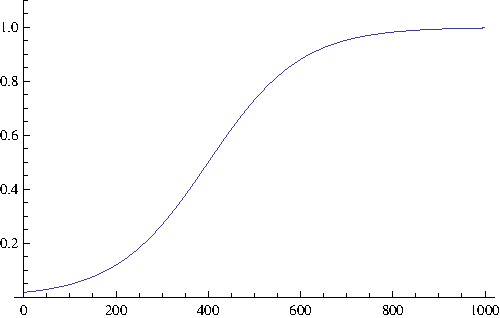
\includegraphics{figures/decision-function.pdf}
\caption{Example of sigmoid function used to decide if keep or not one individual. On the $x$ axis there is the individual rank. With this function the population size will average 400 individuals (our maximum population size in most tests).}
\label{fig:sigmoid}
\end{figure}

In fact, consider the tails of the sigmoid: here the function takes values very close to zero, or very close to one (exponentially close). This implies that fittest individuals always survive and that worst individuals always get killed. In our case, non halting machines are always dropped, because they are normally in the back of the ranking. Non halting machines are important for us, because our aim is to find machines that are \textit{almost} non halting.
Using other functions it's possible, but it remains a problem to have a very low pressure selection and keep the population size under control (not going to zero or infinity).

In order to solve this problem we had also to redesign the fitness function (to give some more importance to this non halting machines), but mainly we had to find some very low pressure selection mechanism.
What we thought is: ``what is the function with the lowest possible selection pressure?''. It is a uniform selection, that is not considering at all the fitness function value. But in this way the search becomes really random, and we don't want this. So we combined this very ``flat'' selection with elitism, and the final selection looks something like this:

\begin{enumerate}
\item Decide a certain number $S$ of individuals to save, for example one fourth of the maximum population size.
\item If the individuals number $N$ is greater than the maximum $M$ the selection happens on the $N-S$ worst individuals. Notice: not $N-M$ (that is only the individuals that exceeds the maximum $M$), but all the individuals that have not been selected by elitism.
\item From this $N-S$ group we kill an average of $N-M$ individuals. We do this iterating over these individuals and test if a random number in $[0,1]$ is smaller than $\frac{N-M}{N-S}$. This means that an individual is removed with probability $\frac{N-M}{N-S}$, that summed over all the $N-S$ scanned individuals gives the wanted average.
\end{enumerate}

Using this selection schema we always have a certain number of not halted machines in the population, so we have very big diversity.

\chapter{Results}
\label{chap:results}

We here show the results we get for different alphabet and states set sizes.

Results are presented in tables where lines are indexed by states and column by symbols. Operational states are called $S_0, S_1, \dots$ for easier reading and $H$ denotes the halt state. To find the transition corresponding to the reading of symbol $s$ in state $e$, look at cell in column $s$ on line $S_e$. The content of this cell is, in order, the symbol to write, the direction where to move the reading head ($L$ stands for \emph{left} and $R$ for \emph{right}) and the state to pass to.

\paragraph{Turing machines with 2 symbols and 2 states}

\begin{itemize}
\item Max-step value \cite{rado}: $S(2,2) = 6$ ;
\item Search space size: 20\,736;
\item Machine we found:
\[
\begin{array}[h]{|c|c|c|}
\hline
   &0     &1\\
\hline
S_0& 0RS_1& 1RH\\
\hline
S_1& 1LS_0& 1RS_1\\
\hline
\end{array}
\]
\item Steps it performs before halting: 6 (so it is a busy beaver).
\end{itemize}

\paragraph{Turing machines with 2 symbols and 3 states}

\begin{itemize}
\item Max-step value: $S(2,3) = 21$;
\item Search space size: 16\,777\,216;
\item Machine we found:
\[
\begin{array}[h]{|c|c|c|c|}
\hline
   & 0    &1\\
\hline
S_0& 1LS_1& 1RH\\
\hline
S_1& 1RS_1& 0LS_2\\
\hline
S_2& 1RS_2& 1RS_0\\
\hline
\end{array}
\]
\item Steps it performs before halting: 21 (so it is a busy beaver).
\end{itemize}


\paragraph{Turing machines with 3 symbols and 2 states}

\begin{itemize}
\item Max-step value: $S(3,2) = 38$;
\item Search space size: 34\,012\,224;
\item Machine we found:
\[
\begin{array}[h]{|c|c|c|c|c|}
\hline
0&   1&   2& 3\\
\hline
S_0& 2LS_1& 0RH& 1RS_1\\
\hline
S_1& 1RS_0& 2RS_1& 1LS_1\\
\hline
\end{array}
\]
\item Steps it performs before halting: 38 (so it is a busy beaver).
\end{itemize}


\paragraph{Turing machines with 2 symbols and 4 states}


\begin{itemize}
\item Max-step value: $S(2,4) = 107$;
\item Search space size: 25\,600\,000\,000;
\item Machine we found:
\[
\begin{array}[h]{|c|c|c|c|}
  \hline
  &0&   1\\
  \hline
  S_0& 1RS_3& 1LS_3\\
  \hline
  S_1& 1LH& 1LS_2\\
  \hline
  S_2& 1RS_2& 0RS_0\\
  \hline
  S_3& 1LS_0& 0LS_1\\
\hline
\end{array}
\]
\item Steps it performs before halting: 107 (so it is a busy beaver).
\end{itemize}

\paragraph{Turing machines with 4 symbols and 2 states}


\begin{itemize}
\item Max-step value: not known but we know [TODO : ref] that $S(2,4) \geq 3\,932\,964$;
\item Search space size: 110\,075\,314\,176;
\item Machine we found at the time of writing:
\[
\begin{array}[h]{|c|c|c|c|c|}
  \hline
&0&   1&   2&   3\\
\hline
  S_0& 1LS_1& 1RS_0& 0RS_1& 1LH\\ 
\hline
  S_1& 3RS_0& 2LS_1& 3LS_0& 1LS_1\\
\hline
\end{array}
\]
\item Steps it performs before halting: 283 (so it is not a busy beaver).
\end{itemize}


\chapter{Outcome}
\label{chap:outcome}


\chapter{Further work}
\label{chap:fwork}

\section{PSO}
We had no time to test a PSO approach, before writing this report. It would be interesting to try it, of course, but we don't think it would be radically different from the current ideas. And in every case it would be a PSO implementation that has to ``jump'', and not ``fly'', over the search space. This happens because the Turing machine's search space is not continuous, and moreover we have to define by ourselves the particle operations that PSO usually performs.

Our search space is made by the genomes we used in the evolutionary computing approach, not vectors. The number of dimensions is the number of free variables in the genome, $3MN$ in total.
In this scenario consider, for example the PSO step where the velocity of a particle is summed up with the current position. How could be implemented this operation on our Turing machines genome? A possible approach [TODO needed citation] is to interpret the velocity as a probability to change the variable corresponding to that dimension.

So it's something very similar to a mutation in the evolutionary computing approach (something in between with a crossover and a mutation actually, since the velocity depends on other particles, other genomes).

We don't want to say that PSO, on this problem, would be the same as using the tool we implemented; it's very difficult to make such prevision, but the ideas will be more or less the same, at least for what concerns this redefinition of the vector operators needed by it.

\section{Optimizations}
A possible optimization regards the virtual machine execution, and in particular it tries to use the following fact:

\begin{Thm}
If a machine $M$ during its execution arrives twice:
\begin{enumerate}
\item in the same state $S$,
\item in the same position on the tape,
\item having the tape unchanged from last time (same size and same content),
\end{enumerate}
means that M will never halt.
\end{Thm}
\begin{proof}
This holds since the transitions are deterministic, so if $M$ showed this behaviour once, it will repeat this infinitely many times.
\end{proof}

In other words this means that $M$ has a ``loop'' of some length $k$ (the number of shifts for going back to the same state $S$). There is a very elegant method for detecting this kind of cycles called Brent's method \cite{brent} (a variant of the Floyd algorithm, credited in \cite{knuth}).

The algorithm keeps track of one previous virtual machine state (so it actually require to double the space occupied by a virtual machine). The algorithm starts saving the state after the first shift. After computing the second shift if checks if the state is the same or not: if it's the same the algorithm just detected a loop, otherwise the virtual machine can compute the next shift. This check happens at every new shift computed by the machine. When the number of shifts is a power of 2, the algorithm stores the current state for the following comparisons.

In this way it's possible to detect loops of any length $k$, if the number of executed shifts is sufficiently large. The nice thing is that detecting a loop not only implies an early stop in a computation that will never end, but also gives more precise informations in terms of fitness function!

But there are of course some drawbacks with this approach:
\begin{enumerate}
\item there is an (increasing) overhead in checking if the current state is equal to the saved one. Increasing because of course the tape size can be bigger and bigger executing the machine.
\item the memory used doubles.
\end{enumerate}

One solution, that also make the algorithm even more effective, is to check not the whole tape, but just a window of it. This of course is an approximation: limiting the check to a certain portion of the tape can lead to wrong decisions (the machine \textit{seems} to have come back to the same state, but it is not).
But of course the bigger is this window, the more precise is this approximation. And having a constant window size, makes the state check constant time (so not increasing with the tape size).

Another solution could be to save an hash of the tape, instead of the full tape. This is very memory effective but, because of the hash collisions can also be inexact. Also a combination of the two approaches would be very interesting to try.



\bibliographystyle{abbrv}
\bibliography{report}

\end{document}